\documentclass[12pt,a4paper]{article}
\usepackage[UTF8]{ctex}
\usepackage{amsmath,amssymb}
\usepackage{xcolor}
\usepackage{hyperref}
\usepackage{geometry}
\usepackage{graphicx}
\geometry{margin=2.5cm}

\title{Amplitude Estimation / 振幅估计}
\author{QuoNic}
\date{}

\begin{document}
\maketitle

\begin{center}
\textbf{Algorithms / 算法} | 难度：高级 | 预计时间：20 分钟
\end{center}

\tableofcontents
\newpage

\section{为什么需要？}

振幅估计用于估计量子算法的成功概率。

\subsection{经典局限}
\begin{itemize}
  \item 经典方法需要多次采样才能估计概率
  \item 对于小概率事件，经典方法效率低
\end{itemize}

\subsection{量子优势}
\begin{itemize}
  \item 振幅估计只需要 $O(1/\epsilon)$ 次查询
  \item 提供二次加速
  \item 是量子算法分析的基础
\end{itemize}

\subsection{实际应用}
\begin{itemize}
  \item 量子算法分析
  \item 量子优化
  \item 量子机器学习
\end{itemize}

\section{快速上手}

\begin{verbatim}
from quonic.algorithms import amplitude_estimation
result = amplitude_estimation(target='11', n_qubits=2)
print(f'Estimate: {result.estimate}')
\end{verbatim}

\textbf{预期输出}：
\begin{verbatim}
Estimate: 0.5
\end{verbatim}

\section{原理详解}

\subsection{电路图}

\begin{center}
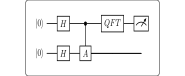
\includegraphics[width=0.6\textwidth]{../../images/amplitude_estimation_circuit.svg}
\end{center}

\subsection{数学推导}

振幅估计结合了振幅放大和量子相位估计：
\begin{equation}
\theta = \arcsin(\sqrt{p})
\end{equation}

其中 $p$ 是目标态的概率。

\textbf{算法步骤}：
\begin{enumerate}
  \item 用振幅放大旋转相位
  \item 用 QPE 估计相位 $\theta$
  \item 计算概率 $p = \sin^2(\theta)$
\end{enumerate}

\subsection{几何解释}

振幅估计在 Bloch 球上估计旋转角度，从而推算成功概率。

\section{代码详解}

\begin{verbatim}
from quonic.algorithms import amplitude_estimation

# amplitude_estimation(target, n_qubits, precision)
# target: target bit string
# n_qubits: number of qubits
# precision: number of precision qubits
result = amplitude_estimation(target='11', n_qubits=2)

# result.estimate: estimated probability
# result.phase: estimated phase
print(f'Estimate: {result.estimate}')
\end{verbatim}

\section{进阶用法}

\subsection{场景 1：不同目标态}

\begin{verbatim}
from quonic.algorithms import amplitude_estimation
result = amplitude_estimation(target='101', n_qubits=3)
print(f'Estimate: {result.estimate}')
\end{verbatim}

\section{适用场景}

\subsection{量子算法分析}

振幅估计可以用于分析量子算法的成功概率。

\subsection{量子优化}

振幅估计可以用于估计优化问题的最优解概率。

\section{常见问题}

\subsection{振幅估计和振幅放大有什么区别？}

振幅估计估计概率，振幅放大放大概率。

\subsection{振幅估计的精度如何？}

精度取决于控制量子比特的数量。更多的控制量子比特提供更高的精度。

\section{学习路径}

\subsection{前置知识}
\begin{itemize}
  \item 振幅放大
  \item 量子相位估计
  \item 量子傅里叶变换
\end{itemize}

\subsection{继续学习}
\begin{itemize}
  \item 量子计数
  \item 量子优化
  \item 量子机器学习
\end{itemize}

\section{完整示例代码}

\subsection{示例 1：基本振幅估计}

\begin{verbatim}
from quonic.algorithms import amplitude_estimation
result = amplitude_estimation(target='11', n_qubits=2)
print(f'Estimate: {result.estimate}')
\end{verbatim}

\section{下载}

\begin{itemize}
  \item [amplitude\_estimation.py](https://github.com/ChrisLee0721/QuoNic/blob/main/examples/amplitude_estimation/amplitude_estimation.py)
\end{itemize}

\end{document}
